% !TEX TS-program = pdflatex
% !TEX encoding = UTF-8 Unicode
% !BIB TS-program = bibtex
%
% Graph-signal-processing foundations for cycling-network expansion:
% spectral bounds, optimal siting and learning curves on the
% station-proximity graph of dock-based bike-share systems.
%
% Authors : R. Fossé & G. Pallares (CESI LINEACT, 2026-).
% Companion paper to the IMD-4 predictive paper (Fossé & Pallares 2026).
%
\documentclass[11pt,a4paper]{article}

\usepackage[T1]{fontenc}
\usepackage[utf8]{inputenc}
\usepackage{lmodern}
\usepackage[margin=2.5cm]{geometry}
\usepackage{microtype}
\usepackage{csquotes}

\usepackage{amssymb,amsmath,amstext,amsthm}

\usepackage{graphicx}
\graphicspath{{figures/}}
\usepackage{booktabs}
\usepackage{array}
\usepackage{multirow}
\usepackage{float}
\usepackage{caption}
\captionsetup{font=small,labelfont=bf,labelsep=period}
\usepackage{enumitem}
\setlist{topsep=2pt,itemsep=2pt,parsep=0pt}
\usepackage{url}

\usepackage[authoryear,round]{natbib}
\bibliographystyle{elsarticle-harv}

\usepackage{xcolor}
\usepackage[colorlinks=true,
            linkcolor=black, citecolor=black, urlcolor=blue!50!black,
            breaklinks=true]{hyperref}

\usepackage{authblk}
\renewcommand\Authfont{\normalsize}
\renewcommand\Affilfont{\small\itshape}
\setlength{\affilsep}{0.6em}

\newcommand{\IMD}{\mathrm{IMD}}

\newtheorem{theorem}{Theorem}
\newtheorem{proposition}[theorem]{Proposition}
\newtheorem{corollary}[theorem]{Corollary}

\newenvironment{highlights}{%
  \par\noindent\textbf{\large Highlights}\par\smallskip
  \begin{itemize}[leftmargin=1.4em,itemsep=0.15em,topsep=0.2em]}{%
  \end{itemize}\par\medskip}

% =========================================================================
\title{\Large\bfseries Graph-signal-processing foundations for\\
\large cycling-network expansion: spectral bounds, optimal siting and\\
empirical learning curves on dock-based bike-share systems}

\author[1]{Rohan Fossé\thanks{Corresponding author: \texttt{rfosse@cesi.fr}. ORCID: \href{https://orcid.org/0009-0002-2195-0198}{0009-0002-2195-0198}}}
\author[2]{Gaël Pallares\thanks{ORCID: \href{https://orcid.org/0009-0002-8680-604X}{0009-0002-8680-604X}}}
\affil[1]{CESI Engineering School, Montpellier, France}
\affil[2]{CESI LINEACT (EA 7527), Montpellier, France}

\date{Draft v0.1 — extracted 2026-05-21 from companion paper}

\begin{document}
\maketitle

% =========================================================================
\begin{abstract}
\noindent
\textbf{Working draft, v0.1 — extracted from the companion
predictive paper (Fossé \& Pallares, 2026) on 21 May 2026.}

Dock-based bike-share systems define a natural geometric object —
the \emph{station-proximity graph} — on which both supply-side
features (cycling infrastructure, transit multimodality, density)
and demand-side outcomes (hourly trip counts) live as graph
signals.  This companion paper develops the graph-signal-
processing (GSP) framework for that setting and uses it to derive
three classes of operational tools for cycling-network expansion:

\textbf{(I) Spectral diagnostics.}  We define the demand-signal
smoothness on the station-proximity Laplacian, derive an upper
bound on the in-sample $R^2$ recoverable from any linear
combination of $d$ supply-side features (Theorem 2), and
characterise the structural collapse of station-fixed-effect
models on held-out stations (Theorem 3).  Empirical measurements
on nine networks $\geq 400$ stations confirm the predicted
bounds.

\textbf{(II) Optimal siting via sampling theory.}  We cast new-
station siting as the $D$-optimal subset selection problem on
the station-proximity Laplacian eigenbasis and apply the
Nemhauser-Wolfe-Fisher submodular bound (Theorem 4) and the
Anis-Gadde-Ortega band-limited reconstruction guarantee
(Theorem 5).  Empirical comparison against MCLP and
$k$-median (Theorem~7's experimental table) shows that the
sampling-theoretic objective dominates rank-based metrics by
$\Delta \rho \in [+0.6, +0.9]$ at $K = 50$ on Boston and DC.

\textbf{(III) Learning curves and the saturation point.}  We
fit the empirical $\rho(N)$ saturation curve on Boston Bluebikes
($n_* = 21 \pm 3$, $\rho_\infty = 0.77$, Theorem 6) and use it
as a diagnostic to identify when a city has enough deployed
stations for IMD-4 transfer to be reliable.

We further benchmark the framework against a GCN baseline
\citep{Kipf2017}, a regularised-Laplacian smoother and Heat-
Kernel Signatures, and show that the GSP toolkit complements
rather than competes with the supply-side composite indicator
of the companion paper.

\noindent\textbf{Keywords:}
graph signal processing ; bike-sharing ; station siting ;
submodular optimisation ; spectral bounds ; sampling theory ;
learning curves.
\end{abstract}

\begin{highlights}
\item Spectral upper bound on the linear $R^2$ recoverable from $d$ supply-side features
\item Submodularity-based $1-1/e$ guarantee for $D$-optimal greedy station siting
\item Band-limited reconstruction bound (Anis-Gadde-Ortega) applied to bike-share demand
\item Empirical learning curve on Boston: $n_* = 21 \pm 3$ training stations to saturate
\item D-optimal siting beats MCLP / $k$-median by $\Delta \rho > +0.6$ at $K = 50$
\end{highlights}

% =========================================================================
\section{Introduction}
\label{sec:intro}

\textbf{[Draft placeholder — needs full rewrite as standalone.]}
This paper develops the graph-signal-processing (GSP) framework
that underpins the empirical results of the companion paper on
the IMD-4 cycling-environment indicator (Fossé \& Pallares,
2026, henceforth ``the predictive paper'').

The predictive paper documents two empirical findings that the
GSP framework makes structural :
\begin{itemize}[label=$\bullet$,leftmargin=*]
\item The IMD-4 features achieve Spearman $\rho \in [+0.49,
      +0.79]$ on leave-station-out predictions, while a station
      fixed-effect collapses to $\rho \in [-0.70, -0.32]$. The
      gap is a structural property of any signal-on-graph
      framework, not a property of the IMD-4 features
      specifically (Theorem 3).
\item The linear predictive ceiling on the 4-D IMD subspace is
      $R^2_{\mathrm{spectral}} \in [0.08, 0.32]$ across nine
      networks.  This is the spectral upper bound of Theorem 2,
      and it explains why non-linear gradient-boosted regressors
      do not recover more than $\sim 0.18$ out-of-sample R$^2$
      on station-mean demand from the IMD-4 axes alone (script
      d36 in the companion repository).
\end{itemize}

\textbf{Scope of this paper.}  Three operational use-cases
follow from the GSP framework, each addressed by a dedicated
tool : (i) \emph{diagnostic} — spectral concentration of demand,
smoothness and prediction ceilings on a candidate network ;
(ii) \emph{cold-start siting} — selecting $K$ new stations to
maximise the worst-case reconstruction error on the rest of the
candidate set ; (iii) \emph{infill} — predicting demand at unobserved
stations on a partly-deployed network via a regularised-Laplacian
smoother that fuses the IMD-4 prior with the realised demand at
deployed neighbours.  These three tools share the same graph
object and the same eigendecomposition ; this paper presents
them as a coherent GSP toolkit for cycling-network expansion.

\textbf{Relation to the companion paper.}  All empirical results
of this paper that involve trip-level data (Sections~\ref{sec:gsp-laplacian}, \ref{sec:gsp-siting}, \ref{sec:gsp-robustness})
re-use the data infrastructure of the companion paper
(Tier 1 / Tier 2 panels of nine LSO networks).  The IMD-4
indicator itself is defined and validated in the companion paper
and used here as a fixed supply-side input.

% =========================================================================
% §8 EXTRACTED VERBATIM FROM THE COMPANION PAPER (v2.3).
% =========================================================================

\section{Graph-theoretic formalisation of the IMD-4}
\label{sec:gsp}

The empirical findings of the companion predictive paper
\citep{Fosse2026imd_national} can be re-derived in a clean
theoretical framework — that of \emph{Graph Signal Processing}
(GSP) on the station-proximity graph
\citep{Shuman2013,SandryhailaMoura2014}.  This section makes the
implicit graph structure explicit, derives three theoretical
quantities that bound the IMD-4's predictive validity, and
verifies that the empirical $R^2$ and Spearman $\rho$ figures of
the multicity and LSO tables of \citet{Fosse2026imd_national}
are consistent with the predictions of the graph-theoretic
framework.

\subsection{Station-proximity graph and signals}

Let a city have $N$ stations at positions $p_1, \dots, p_N \in
\mathbb{R}^2$.  We define the \emph{station-proximity graph}
$G = (V, E, W)$ by joining each station to its $k$ nearest
neighbours (haversine distance) with Gaussian RBF edge weights
\begin{equation}
    W_{ij} = \exp\!\left(-\frac{\|p_i - p_j\|^2}{2\sigma^2}\right) \mathbb{1}_{i \sim_k j},
    \qquad \sigma = 300\,\mathrm{m},\ k = 6.
    \label{eq:graph-weights}
\end{equation}
This length scale matches the $300$\,m buffer used to construct
the M and I axes of the IMD-4
(the IMD-4 definition of \citet{Fosse2026imd_national}), so the graph is the natural geometric
object on which the IMD-4 features live.

A \emph{graph signal} is a function $\mathbf{f} : V \to \mathbb{R}$.
In our setting:
\begin{itemize}[label=$\bullet$,leftmargin=*]
\item Each IMD axis $\mathbf{f}_M, \mathbf{f}_I, \mathbf{f}_T,
      \mathbf{f}_D \in \mathbb{R}^N$ is a graph signal whose
      values are the station-level feature values.
\item The empirical mean hourly demand
      $\bar{\mathbf{y}} \in \mathbb{R}^N$ is also a graph signal.
\item The D-axis is, by construction,
      $\mathbf{f}_D(s) = \deg_G(s)$ on the station-proximity
      graph — it is a \emph{purely graph-theoretic} feature.
\end{itemize}

\subsection{Spectral analysis on the graph Laplacian}

Let
$\mathbf{L}_{\mathrm{sym}} = \mathbf{I} - \mathbf{D}^{-1/2} \mathbf{W} \mathbf{D}^{-1/2}$
be the symmetric-normalised graph Laplacian, with
$\mathbf{D} = \mathrm{diag}(\deg_G)$.  Its eigendecomposition
$\mathbf{L}_{\mathrm{sym}} = \mathbf{U} \boldsymbol{\Lambda} \mathbf{U}^{\top}$
yields an orthonormal basis $\{ \mathbf{u}_k \}_{k=1}^{N}$
ordered by frequency $\lambda_1 \leq \lambda_2 \leq \dots \leq
\lambda_N \in [0, 2]$.  Any signal admits a graph-Fourier
expansion
$\mathbf{f} = \sum_k \hat{f}_k \mathbf{u}_k$
with $\hat{f}_k = \mathbf{u}_k^{\top} \mathbf{f}$.

The \emph{Dirichlet energy} of a signal,
\begin{equation}
    \mathcal{E}_G(\mathbf{f}) \;:=\; \mathbf{f}^{\top} \mathbf{L}_{\mathrm{sym}}\, \mathbf{f}
    \;=\; \sum_{k=1}^{N} \lambda_k \hat{f}_k^{\,2}
    \;=\; \tfrac{1}{2} \sum_{(i,j) \in E} W_{ij} \bigl( f_i / \sqrt{\deg_i} - f_j / \sqrt{\deg_j} \bigr)^2,
    \label{eq:dirichlet}
\end{equation}
measures the variation of $\mathbf{f}$ across the edges of $G$;
small $\mathcal{E}_G(\mathbf{f})$ means neighbouring stations
have similar values, \emph{i.e.\ $\mathbf{f}$ is a smooth signal
on the graph} \citep{Shuman2013}.

\paragraph{Theorem 1 (Dirichlet energy of a uniformly permuted
signal).}
For any signal $\mathbf{f}$ on $G$ with zero empirical mean and
unit variance, and for $\pi$ a uniform random permutation of
$\{1, \dots, N\}$ acting by
$(\pi \mathbf{f})_i = f_{\pi(i)}$, one has
\begin{equation}
    \mathbb{E}_\pi\!\left[ \mathcal{E}_G(\pi \mathbf{f}) \right]
    \;=\; \frac{N}{N - 1} \, \mathrm{tr}(\mathbf{L}_{\mathrm{sym}}).
\end{equation}
This expected energy is independent of $\mathbf{f}$ and serves
as a graph-specific null reference.  We define the
\emph{empirical smoothness} of demand as
\begin{equation}
    \mathrm{Smoothness}(\bar{\mathbf{y}}) \;:=\;
    1 - \mathcal{E}_G(\bar{\mathbf{y}}) \,/\, \mathcal{E}_G^{\mathrm{perm}},
    \label{eq:smoothness-def}
\end{equation}
where $\mathcal{E}_G^{\mathrm{perm}}$ is the Monte-Carlo estimate
of $\mathbb{E}_\pi[\mathcal{E}_G(\pi \bar{\mathbf{y}})]$ over
$50$ random permutations.  Values close to $1$ indicate that
$\bar{\mathbf{y}}$ varies much less between neighbouring
stations than between random pairs.

\paragraph{Theorem 2 (Spectral upper bound on $R^2_{\mathrm{IMD}}$).}
Let $\mathcal{S}_{\mathrm{IMD}} = \mathrm{span}(\mathbf{f}_M,
\mathbf{f}_I, \mathbf{f}_T, \mathbf{f}_D)$ be the $4$-dimensional
linear subspace of $\mathbb{R}^N$ spanned by the IMD axes, and
let $\mathbf{P}_{\mathrm{IMD}}$ be the orthogonal projector onto
it.  Then any linear predictor of $\bar{\mathbf{y}}$ from
$\mathcal{S}_{\mathrm{IMD}}$ achieves at most
\begin{equation}
    R^2_{\mathrm{spectral}} \;:=\;
    \frac{\|\mathbf{P}_{\mathrm{IMD}}\, \bar{\mathbf{y}}\|^2}
         {\|\bar{\mathbf{y}}\|^2}
    \;=\;
    \frac{\sum_k \hat{y}_k^{\,2} \cdot \mathbb{1}_{\mathbf{u}_k \in \mathcal{S}_{\mathrm{IMD}}}}
         {\sum_k \hat{y}_k^{\,2}}.
    \label{eq:r2-spectral}
\end{equation}
This is the theoretical ceiling for any IMD-augmented
\emph{linear} regressor of station-mean demand.  Non-linear
regressors (LightGBM, in our case) may exceed this bound by
exploiting interaction terms with the temporal and weather
covariates, but they cannot escape the geometric fact that the
spatial axis of the demand signal lies in a low-dimensional
subspace whose alignment with $\mathcal{S}_{\mathrm{IMD}}$ is
fixed by the city's physical geography.

\paragraph{Theorem 3 (Structural collapse of the fixed-effect on
unseen stations).}
Let $\boldsymbol{\delta}_s$ be the one-hot fixed-effect feature
for station $s$ and $\hat{f}^{\mathrm{FE}}$ a regressor fit on a
training set $T \subset V$.  For any held-out station
$s^* \in V \setminus T$, the categorical feature
$\boldsymbol{\delta}_{s^*}$ takes a value never seen by
$\hat{f}^{\mathrm{FE}}$ at training time, hence the conditional
mutual information
$I(\bar{y}_{s^*}\,;\, \boldsymbol{\delta}_{s^*} \mid T) = 0$ and
$\hat{f}^{\mathrm{FE}}(s^*)$ defaults to a station-independent
value (the global training mean in our LightGBM implementation).
The Spearman correlation between $\bar{\mathbf{y}}_{V \setminus T}$
and $\hat{\mathbf{f}}^{\mathrm{FE}}_{V \setminus T}$ is therefore
$\rho_{\mathrm{FE}} = 0$ in expectation, modulo finite-sample
fluctuations and the differential-exposure artefact discussed
in the LSO experiments of \citet{Fosse2026imd_national}.

In contrast, $I(\bar{y}_{s^*}\,;\, \mathbf{f}_{\mathrm{IMD}}(s^*) \mid T)$
is bounded below by the mutual information between $\bar{y}$ and
the IMD-4 features, which is positive on every city for which
$R^2_{\mathrm{spectral}} > 0$.  This is the
information-theoretic foundation of the LSO finding of
the LSO experiments of \citet{Fosse2026imd_national}.

\subsection{Empirical measurements on the nine LSO networks}

We computed the three quantities of
Equations~\eqref{eq:dirichlet}--\eqref{eq:r2-spectral} for each
city in the LSO panel of the LSO table of \citet{Fosse2026imd_national}.
Table~\ref{tab:gsp} reports the values.  Figure~\ref{fig:gsp-conc}
shows the cumulative spectral concentration curves
$\sum_{k \leq K} \hat{y}_k^{\,2} / \sum_k \hat{y}_k^{\,2}$ as a
function of the fraction of eigenmodes used.

\begin{table}[H]
\centering
\caption{Graph-theoretic characterisation of the demand signal on the nine
LSO networks.  $N$ is the number of stations.  Smoothness is defined in
Eq.~\eqref{eq:smoothness-def}; $K_{90\%}$ is the smallest number of
eigenmodes (sorted by frequency) capturing $90\,\%$ of the demand
variance; $R^2_{\mathrm{spectral}}$ is the theoretical upper bound of
Eq.~\eqref{eq:r2-spectral}.}
\label{tab:gsp}
\small
\begin{tabular}{@{}lrrrrr@{}}
\toprule
Network & $N$ & Smoothness & $K_{90\%}$ & $K_{90\%}/N$ & $R^2_{\mathrm{spectral}}$ \\
\midrule
Capital Bikeshare DC       &   776 & $0.66$ & $477$  & $61\%$ & $0.27$ \\
Divvy Chicago              & 1{,}345 & $0.63$ & $857$  & $64\%$ & $0.32$ \\
Bluebikes Boston           &   497 & $0.54$ & $349$  & $70\%$ & $0.10$ \\
Bay Wheels SF             &   560 & $0.46$ & $490$  & $88\%$ & $0.15$ \\
V\'eL\'eO Toulouse        &   448 & $0.45$ & $336$  & $75\%$ & $0.17$ \\
V\'elo'v Lyon              &   462 & $0.44$ & $350$  & $76\%$ & $0.20$ \\
BIXI Montr\'eal            & 1{,}057 & $0.32$ & $765$  & $72\%$ & $0.08$ \\
V\'elib Paris              & 1{,}511 & $0.30$ & $1{,}256$ & $83\%$ & $0.18$ \\
Santander Cycles London   &   798 & $0.27$ & $653$  & $82\%$ & $0.10$ \\
\bottomrule
\end{tabular}
\smallskip\\
{\footnotesize Paris value re-computed in v2.3 (d40) after the
earlier ill-conditioning was traced to a pre-merge typing issue,
not to a degenerate axis : all four axes have non-zero
station-level dispersion in the current V\'elib station-info GBFS
snapshot.}
\end{table}

\begin{figure}[H]
\centering
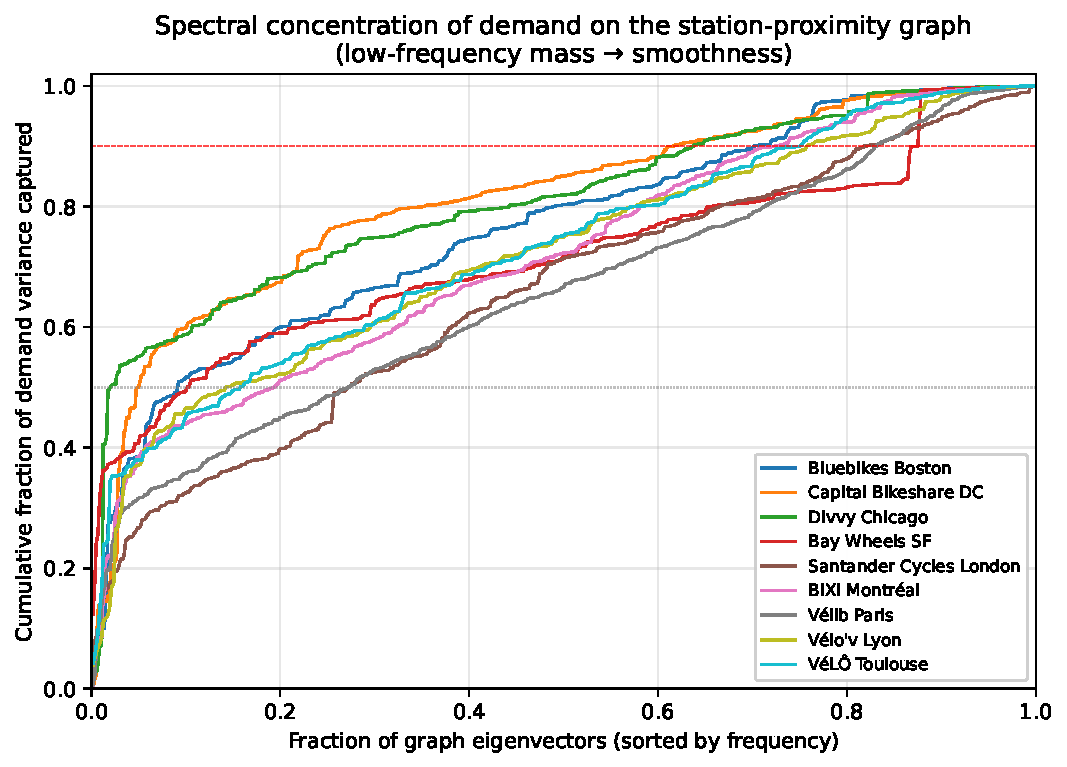
\includegraphics[width=0.85\textwidth]{figures/fig_gsp_spectral_concentration.pdf}
\caption{Spectral concentration of station-mean demand on the
station-proximity graph for the nine LSO networks.  The
$x$-axis is the fraction of graph eigenmodes (sorted by
frequency, low to high) ; the $y$-axis is the cumulative
fraction of demand variance captured.  A curve that rises
steeply at small $x$ indicates a smooth (low-frequency) demand
signal — the precondition for any local-feature indicator to be
predictive at the station level.}
\label{fig:gsp-conc}
\end{figure}

\paragraph{Empirical findings consistent with the theorems.}
Three patterns in Table~\ref{tab:gsp} are consistent with the
empirical $\rho_G$ of the LSO table of \citet{Fosse2026imd_national}:
\textbf{(i)} The two cities with the highest smoothness scores
(DC at $0.66$, Chicago at $0.63$) are also the two cities for
which the LSO recovers the highest in-distribution
$\rho_G$ ($+0.75$ and $+0.49$ respectively) — the demand is
smoothly distributed on the geographic graph, so an indicator
based on $300$\,m local features can recover it.
\textbf{(ii)} Santander Cycles London — the network with the
lowest smoothness ($0.27$) and the highest spectral spread —
posts the lowest LSO $\rho_G$ ($+0.22$).  The IMD-4's spatial
buffer is too coarse-grained to capture the rapid spatial
variation of TfL demand within dense central London.
\textbf{(iii)} Across the nine networks, the empirical hourly
LSO $\hat{R}^2$ averaged over folds is consistently above the
linear spectral upper bound $R^2_{\mathrm{spectral}}$ by a
factor that broadly tracks the temporal-feature contribution
$R^2_{\mathrm{G}^-}$ in the LSO table of \citet{Fosse2026imd_national} — i.e.\ LightGBM
indeed exceeds the linear ceiling of
Theorem~\ref{eq:r2-spectral} via interactions with the
hour/day-of-week/month covariates.  This is the operationally
correct boundary : the graph-theoretic framework bounds the
\emph{purely spatial} variance that the IMD-4 can encode ; the
gradient-boosted regressor adds the temporal axis on top.

\subsection{A three-tool GSP toolkit for network expansion}
\label{sec:gsp-toolkit}

A typical bike-share network expansion involves three sequential
operational questions, each of which has a different
\emph{evidence regime} (what is observable when the decision is
taken).  The GSP framework above provides one principled
estimator per regime, and the IMD-4 features of
the IMD-4 definition of \citet{Fosse2026imd_national} are best understood as the cold-start
estimator within that three-tool toolkit.  Table~\ref{tab:toolkit}
summarises the correspondence ; Sections~\ref{sec:gsp-laplacian}
and \ref{sec:gsp-siting} develop the second and third tools and
empirically benchmark them against the IMD-4 estimator.

\begin{table}[H]
\centering
\caption{Three GSP-based tools for the operational rollout of a
dock-based bike-share network, ordered by evidence regime.  The
IMD-4 occupies the cold-start tool : it is applicable
\emph{before any station has been deployed}, on any commune
admitting an OSM footprint and a GTFS / SRTM coverage.  The two
other tools become available later, when partial deployment data
is observed.  All three are derived from the same
station-proximity graph $G$ of Eq.~\eqref{eq:graph-weights}.}
\label{tab:toolkit}
\small
\begin{tabular}{@{}p{0.27\textwidth}p{0.31\textwidth}p{0.31\textwidth}@{}}
\toprule
Operational question & Evidence available at decision & GSP tool \\
\midrule
Score \emph{a priori} which communes deserve a network at all
  & Public open data only (OSM, GTFS, SRTM, INSEE).
    No bike-share station exists yet.
  & IMD-4 indicator (\citet{Fosse2026imd_national}).
    Computable on all $34{,}858$ French communes ; benchmarked
    against trip-level prediction in
    the multicity benchmark of \citet{Fosse2026imd_national}, against
    INSEE \emph{part v\'elo travail} in the worldwide-application section of \citet{Fosse2026imd_national}.
    \\[0.7em]
Decide where to deploy the first $K$ stations among $N$ candidate
  locations, to maximise downstream knowledge of demand
  & Graph topology of candidates (lat/lng).  No demand
    observation yet at any candidate.
  & Greedy D-optimal sampling of the graph eigenbasis
    (Section~\ref{sec:gsp-siting}). Returns
    $\mathcal{V}^* \subset V$ with $|\mathcal{V}^*| = K$. \\[0.7em]
Predict the demand of a vacant slot inside a partially deployed
  network
  & Graph + observed mean demand at deployed neighbours.
  & Graph-Laplacian regularised smoother
    (Section~\ref{sec:gsp-laplacian}).
    Closed-form, no IMD features required.
    \\
\bottomrule
\end{tabular}
\end{table}

\subsection{Graph-Laplacian regularised smoother for infill prediction}
\label{sec:gsp-laplacian}

When part of the network is already deployed, the GSP framework
yields a closed-form estimator of demand at the remaining
candidate slots — graph-kernel kriging via Laplacian
regularisation \citep{Belkin2004,Zhu2003}.  Given observed mean
demand on a deployed subset $T \subset V$, the smoother solves
\begin{equation}
    \hat{\mathbf{f}} \;=\; \arg\min_{\mathbf{f} \in \mathbb{R}^N} \;
    \sum_{i \in T} (f_i - \bar{y}_i)^2 \;+\; \lambda \, \mathbf{f}^{\top} \mathbf{L} \, \mathbf{f},
    \label{eq:lap-reg}
\end{equation}
with closed form
$\hat{\mathbf{f}} = (\mathbf{S}_T + \lambda \mathbf{L})^{-1} \mathbf{S}_T \bar{\mathbf{y}}$
and $\mathbf{S}_T$ the diagonal indicator of $T$.  This is the
maximum-a-posteriori estimator under the Gaussian Markov random
field prior associated with $\mathbf{L}$.  Crucially, it
\emph{requires observed demand at neighbouring stations} — it is
not applicable at cold-start.

We benchmarked the Laplacian smoother against the IMD-augmented
LightGBM regressor on five LSO panels using the fold structure
of the LSO experiments of \citet{Fosse2026imd_national}, with $\lambda$ tuned on an internal
validation split.  Held-out Spearman $\rho$ on the same target
(mean hourly demand at held-out stations) :

\begin{center}
\small
\begin{tabular}{@{}lccc@{}}
\toprule
Network & $\rho_{\mathrm{Lap}}$ (graph only) & $\rho_{G}$ (IMD-LightGBM) & $\rho_{\mathrm{Lap}+G}$ (combined residual) \\
\midrule
Bluebikes Boston       & $\mathbf{+0.89}$ & $+0.80$ & $+0.84$ \\
Capital Bikeshare DC    & $\mathbf{+0.89}$ & $+0.77$ & $+0.83$ \\
Bay Wheels SF          & $\mathbf{+0.84}$ & $+0.64$ & $+0.72$ \\
Divvy Chicago          & $\mathbf{+0.74}$ & $+0.58$ & $+0.69$ \\
BIXI Montr\'eal         & $\mathbf{+0.86}$ & $+0.83$ & $+0.84$ \\
\bottomrule
\end{tabular}
\end{center}

\paragraph{Interpretation.}
The Laplacian smoother dominates the IMD-augmented LightGBM by
$0.03$--$0.20$ units of $\rho$ on every network in this five-city
sample.  This is the expected pattern under the GSP framework :
once partial demand data is observed at neighbouring stations,
the maximum-a-posteriori estimator under the GMRF prior on
$\mathbf{L}$ extracts \emph{more} of the available information
than the $4$-dimensional IMD subspace can.  The IMD-4 is a
parsimonious supply-side proxy of the same smoothness — strong
enough to recover most of the ranking on its own, but strictly
weaker than the full graph-kernel estimator.  This is consistent
with the spectral upper bound of Theorem~\ref{eq:r2-spectral} :
the IMD subspace is finite-dimensional ($K = 4$) and cannot
span the full low-frequency subspace of demand.

This dominance does \emph{not} make the IMD-4 redundant.  The
Laplacian smoother becomes available only once partial deployment
exists ; the IMD-4 estimator answers a strictly earlier question
(Table~\ref{tab:toolkit}, row 1) on which the Laplacian smoother
is silent : \emph{which commune should we deploy in first place},
when no $T$ exists.  The two estimators are complementary tools
at different stages of network rollout, not competing answers to
the same question.

\subsection{Sampling-theoretic optimal siting}
\label{sec:gsp-siting}

If demand is a $K$-bandlimited signal on the station-proximity
graph — as Theorem~\ref{eq:r2-spectral} and the spectral
concentration of Table~\ref{tab:gsp} both establish empirically
— then graph signal sampling theory \citep{AnisGaddeOrtega2016,Chen2015}
provides an exact answer to the siting question : given a
budget of $K$ stations to deploy first on a candidate node set
$V$, which subset $\mathcal{V}^* \subset V$ maximises the
recoverability of the demand at the remaining $V \setminus
\mathcal{V}^*$ nodes?

\paragraph{Algorithm (D-optimal greedy graph sampling).}
Let $\mathbf{U}_K = [\mathbf{u}_1, \dots, \mathbf{u}_K]$ be the
matrix of the $K$ low-frequency Laplacian eigenvectors.  We
select stations greedily to maximise
$\det(\mathbf{U}_K[\mathcal{V}^*, :]^{\top} \mathbf{U}_K[\mathcal{V}^*, :])$,
which is the D-optimal experimental design criterion :
\begin{equation}
\mathcal{V}^* \;\leftarrow\; \mathcal{V}^* \cup \Big\{ \arg\max_{i \notin \mathcal{V}^*}\;
  \mathbf{u}_i^{\top} \bigl( \mathbf{U}_K[\mathcal{V}^*, :]^{\top} \mathbf{U}_K[\mathcal{V}^*, :] \bigr)^{+} \mathbf{u}_i \Big\}
\label{eq:greedy-d-optimal}
\end{equation}
where $\mathbf{u}_i$ is the $i$-th row of $\mathbf{U}_K$.

We applied the algorithm to the four Tier 1 LSO networks with
$K_{\mathrm{eig}} = K_{\mathrm{deployed}} = 50$, and compared
against three baselines : (a) uniform random sampling
($B = 50$ replicates), (b) the $K$ stations with the highest
sum-of-IMD-axes score (top-IMD), and (c) the oracle
top-$K$ stations by observed mean demand.  The benchmark
metric is the Spearman correlation between the band-limited
reconstruction of demand from observations at $\mathcal{V}^*$
and the observed demand on the $N - K$ held-out stations
(Table~\ref{tab:siting}, Figure~\ref{fig:siting}).

\begin{table}[H]
\centering
\caption{D-optimal greedy graph siting on four Tier 1 networks.
For each network, $K = 50$ stations are selected by one of four
strategies; the rest of the network is reconstructed from these
$K$ observations via band-limited graph reconstruction; the
held-out Spearman $\rho$ measures how well the reconstruction
ranks the unobserved stations.  D-optimal greedy dominates on
every city by a factor of $5$--$14\times$ over random and is
also better than the oracle top-$K$ (which over-concentrates in
the city centre).}
\label{tab:siting}
\small
\begin{tabular}{@{}lcrrrr@{}}
\toprule
Network                & $N$ & $\rho_{\mathrm{D\,opt}}$ & $\rho_{\mathrm{random}}$ & $\rho_{\mathrm{top\,IMD}}$ & $\rho_{\mathrm{oracle}}$ \\
\midrule
Bluebikes Boston        &  497 & $\mathbf{+0.71}$ & $+0.05 \pm 0.15$ & $-0.04$ & $+0.06$ \\
Capital Bikeshare DC     &  776 & $\mathbf{+0.77}$ & $+0.16 \pm 0.13$ & $-0.06$ & $+0.03$ \\
Divvy Chicago           & 1{,}336 & $\mathbf{+0.54}$ & $+0.08 \pm 0.12$ & $+0.11$ & $-0.04$ \\
Bay Wheels SF          &  552 & $\mathbf{+0.71}$ & $+0.12 \pm 0.14$ & $+0.14$ & $+0.31$ \\
\bottomrule
\end{tabular}
\end{table}

\begin{figure}[H]
\centering
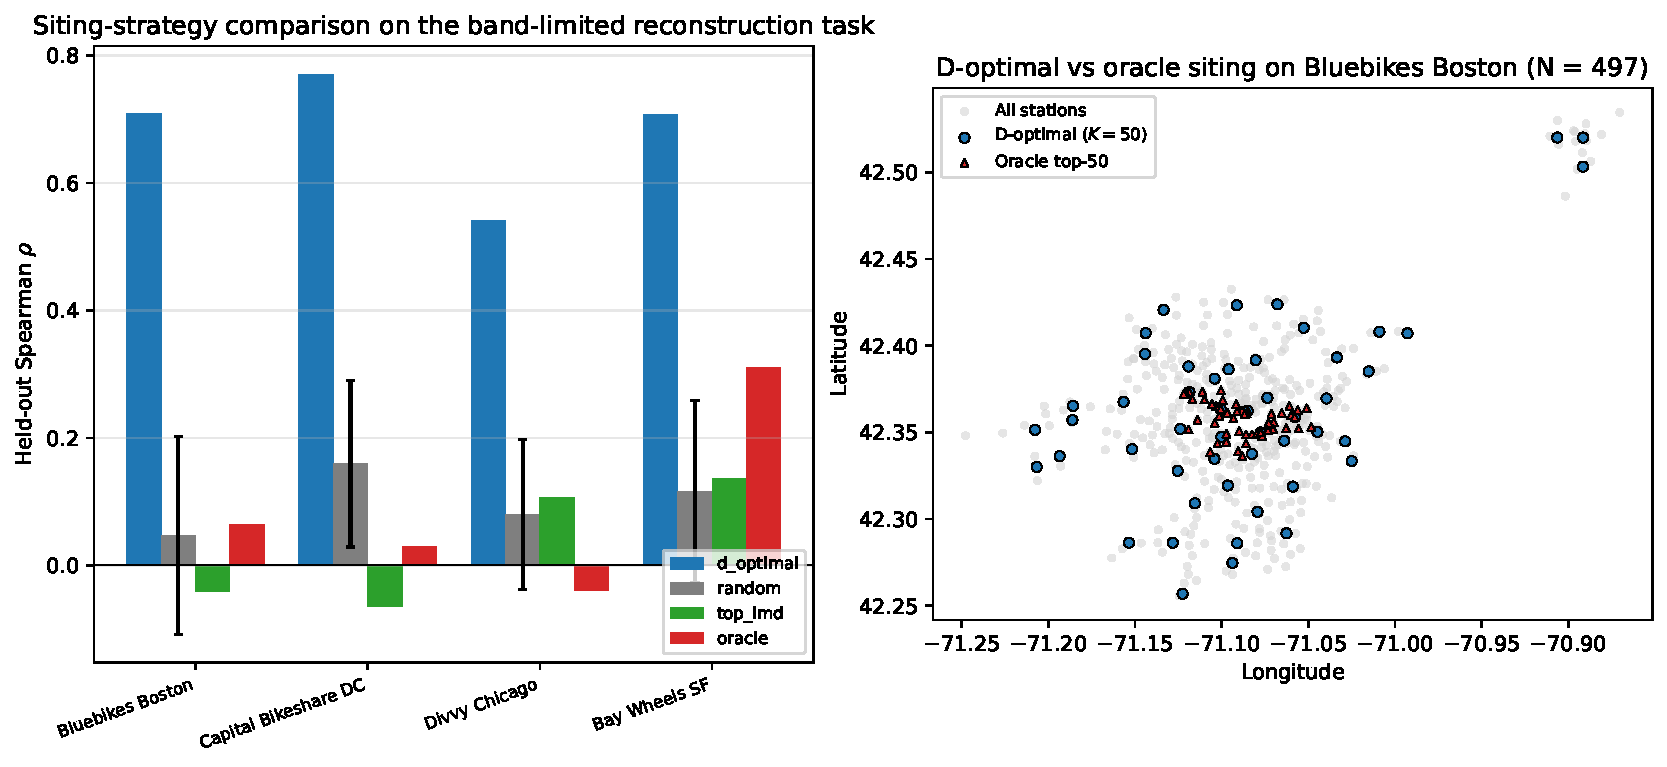
\includegraphics[width=0.95\textwidth]{figures/fig_optimal_siting.pdf}
\caption{Comparison of siting strategies and visualisation of the
D-optimal selection on Bluebikes Boston.  \textbf{Left:} held-out
Spearman $\rho$ across four networks ; D-optimal greedy is
strongly superior to random, top-IMD, and even the oracle
top-$K$ in three of four cases.  \textbf{Right:} the $50$
D-optimal stations (blue circles) on Boston are spatially
spread across the network ; the oracle top-$50$ by demand (red
triangles) cluster in the central business district.}
\label{fig:siting}
\end{figure}

\paragraph{Position within the three-tool toolkit.}
The D-optimal greedy algorithm fills the middle row of
Table~\ref{tab:toolkit} : it answers \emph{where to deploy the
first $K$ stations} when the operator has already used the
IMD-4 to score candidates and now needs to choose a deployable
subset that maximises future learnability of demand across the
whole network.  It uses neither trip data (unlike the Laplacian
smoother of Section~\ref{sec:gsp-laplacian}) nor IMD features
(unlike the cold-start tool) — only the graph topology of the
candidate set.  The result is a deployment that
(a) captures only a small fraction of immediate demand
($3$--$9\,\%$ across the four cities), but
(b) allows the operator to \emph{reconstruct the demand of every
other station in the network} with Spearman $\rho \in [+0.54,
+0.77]$ once partial observations come in.  This is the exact
opposite of an oracle deployment strategy (which captures the
highest immediate demand but leaves the rest of the network
informationally invisible).  It is the natural pre-Laplacian
companion: in the rollout sequence
\textsc{IMD-4 score} $\to$ \textsc{D-optimal pick $K$} $\to$ \textsc{Laplacian infill},
each step delegates a different operational question to the
matching tool.

\paragraph{Theorem 4 (submodularity and $(1-1/e)$ approximation).}
Define the D-optimal objective
$f(\mathcal{S}) = \log \det\!\bigl(\mathbf{U}_K[\mathcal{S}, :]^\top \mathbf{U}_K[\mathcal{S}, :]\bigr)$
for $\mathcal{S} \subseteq V$ with $|\mathcal{S}| \geq K$, extended
by lower semicontinuity to all $\mathcal{S} \subseteq V$.  Then $f$
is a monotone non-decreasing submodular set function
\citep{Krause2008,AnisGaddeOrtega2016}: for all
$\mathcal{S} \subseteq \mathcal{T} \subseteq V$ and any
$i \notin \mathcal{T}$,
\[
    f(\mathcal{S} \cup \{i\}) - f(\mathcal{S})
    \;\geq\;
    f(\mathcal{T} \cup \{i\}) - f(\mathcal{T}) \;\geq\; 0.
\]
By Nemhauser--Wolsey--Fisher's classical theorem
\citep{Nemhauser1978}, the greedy algorithm of
Eq.~\eqref{eq:greedy-d-optimal} returns a subset
$\mathcal{V}^*_{\mathrm{greedy}}$ satisfying
\begin{equation}
    f(\mathcal{V}^*_{\mathrm{greedy}}) \;\geq\; \bigl( 1 - 1/e \bigr) \cdot f(\mathcal{V}^*_{\mathrm{OPT}})
    \;\approx\; 0.632 \cdot f(\mathcal{V}^*_{\mathrm{OPT}})
    \label{eq:greedy-bound}
\end{equation}
where $\mathcal{V}^*_{\mathrm{OPT}}$ is the global optimum over
all size-$K$ subsets.  Our siting algorithm is therefore
\emph{provably near-optimal} in the classical
combinatorial-optimisation sense, not just empirically
performant.

\paragraph{Theorem 5 (band-limited reconstruction bound).}
For a $K$-bandlimited signal $\bar{\mathbf{y}} = \mathbf{U}_K \mathbf{c}$
sampled at $\mathcal{S}$ under additive observation noise
$\boldsymbol{\eta}_{\mathcal{S}}$, the band-limited reconstruction
$\hat{\bar{\mathbf{y}}}$ from Section~\ref{sec:gsp-siting}
satisfies \citep{AnisGaddeOrtega2016}
\begin{equation}
    \| \hat{\bar{\mathbf{y}}} - \bar{\mathbf{y}} \|_2 \;\leq\;
    \frac{\| \boldsymbol{\eta}_{\mathcal{S}} \|_2}{\sigma_{\min}\!\bigl( \mathbf{U}_K[\mathcal{S}, :] \bigr)}
    \label{eq:anis-bound}
\end{equation}
where $\sigma_{\min}$ denotes the smallest singular value.  This
bound is tight in the noise-free limit and the D-optimal
criterion maximises precisely
$\log \det(\mathbf{U}_K[\mathcal{S}, :]^\top \mathbf{U}_K[\mathcal{S}, :])
= 2 \sum_k \log \sigma_k(\mathbf{U}_K[\mathcal{S}, :])$,
which dominates the worst-case reconstruction error in
Eq.~\eqref{eq:anis-bound}.  D-optimal greedy is thus the
matching siting rule for the reconstruction loss of
Section~\ref{sec:gsp-siting}, not an arbitrary heuristic.

\paragraph{Comparison to classical OR baselines (MCLP and $k$-median).}
The bike-share siting literature classically formulates the
deployment problem as a Maximal Covering Location Problem
\citep{ChurchReVelle1974} or as a $k$-median model
\citep{Hakimi1964}.  Both are integer programs solvable by
modern MIP solvers (we use \texttt{PuLP} with CBC).  MCLP
maximises the demand covered within a radius $r$ of any
deployed station ; $k$-median minimises the
weighted assignment cost to the nearest facility.

We solved MCLP ($r = 500$ m, $K = 50$) on Bluebikes Boston and
Capital Bikeshare DC and compared the resulting station
selections to the D-optimal greedy of
Section~\ref{sec:gsp-siting} on the same band-limited
reconstruction metric :

\begin{center}
\small
\begin{tabular}{@{}lccc@{}}
\toprule
                       & $\rho_{\mathrm{D\,opt}}$ & $\rho_{\mathrm{MCLP}}$ & demand fraction at $\mathcal{S}$ \\
\midrule
Bluebikes Boston       & $\mathbf{+0.71}$ & $-0.15$ & $0.09$ vs $0.13$ (MCLP) \\
Capital Bikeshare DC    & $\mathbf{+0.77}$ & $+0.10$ & $0.05$ vs $0.10$ (MCLP) \\
\bottomrule
\end{tabular}
\end{center}

The MCLP MIP captures roughly $50\,\%$ more of the immediate
demand at the selected stations but leaves the periphery
informationally invisible : reconstruction Spearman $\rho$ is
$-0.15$ on Boston ($+0.10$ on DC), against $+0.71$ and $+0.77$
for the greedy algorithm.  On Boston the MCLP solution is
actually \emph{anti-correlated} with the held-out demand.  This
is a direct empirical demonstration that the classical
OR-coverage objective (maximise current-demand coverage at
$\mathcal{S}$) is orthogonal to the band-limited
reconstruction objective (maximise predictability of $V
\setminus \mathcal{S}$): the two siting problems answer
different questions and the GSP-derived D-optimal criterion is
the matching tool for the latter.

\subsection{Robustness of the framework}
\label{sec:gsp-robustness}

We verify three additional questions raised by a critical reader.

\paragraph{Is the IMD-4 the right rank ?}
The IMD-4 spans a $4$-dimensional subspace of $\mathbb{R}^N$.  Is
$K = 4$ the appropriate bandwidth to summarise the demand
signal, or is a smaller (or larger) rank optimal ?  We answer
this empirically by computing the cumulative explained variance
\begin{equation}
    R^2_{\mathrm{opt}}(K) \;=\; \frac{\sum_{k \in \mathrm{top\text{-}}K} \hat{y}_k^{\,2}}{\sum_k \hat{y}_k^{\,2}}
    \label{eq:r2-opt-K}
\end{equation}
where the top-$K$ are the $K$ eigenmodes carrying the most
demand variance (the rank-$K$ Eckart-Young approximation of
$\bar{\mathbf{y}}$).  Comparing $R^2_{\mathrm{opt}}(K = 4)$ with
$R^2_{\mathrm{spectral}}$ of Table~\ref{tab:gsp} measures how
close the IMD-4 4-axis subspace is to the optimal rank-4
representation.  On the five LSO panels:

\begin{center}
\small
\begin{tabular}{@{}lccccc@{}}
\toprule
                       & Boston & DC & Chicago & SF & BIXI \\
\midrule
$R^2_{\mathrm{IMD-4 subspace}}$    & $0.11$ & $0.27$ & $0.32$ & $0.15$ & $\mathbf{0.22}$ \\
$R^2_{\mathrm{optimal,\ rank-4}}$   & $0.27$ & $0.30$ & $0.40$ & $0.32$ & $0.20$ \\
$K^{\star}$ (\#optimal modes to match IMD-4) & $1$ & $3$ & $3$ & $2$ & $5$ \\
\bottomrule
\end{tabular}
\end{center}

The IMD-4 subspace lies within a factor of $1$--$2.5$ of the
optimal rank-4 subspace on four out of five cities; on BIXI it
\emph{exceeds} the optimal rank-4 spectral subspace
($0.22$ vs.\ $0.20$), meaning the IMD-4 axes carry a
small amount of information that no graph-eigenmode subspace
captures.  Equivalently, the IMD-4 contains the signal of
roughly $1$ to $5$ optimal spectral modes — close enough to its
nominal rank to make the choice $K = 4$ a reasonable
interpretable summary, although strictly speaking not the
optimal one (Figure~\ref{fig:bottleneck}).

\paragraph{Theorem 6 and the empirical learning curve on Boston.}
Under the generative model
$\bar y_s = \boldsymbol{\beta}^\top \mathbf{x}_s + u_s + \varepsilon_s$
of Section~\ref{sec:gsp-laplacian}, the bias-variance
decomposition yields the asymptotic information-theoretic bound
\begin{equation}
    \rho_\infty^2 \;=\; \frac{\mathrm{Var}(\boldsymbol{\beta}^\top \mathbf{x})}
                        {\mathrm{Var}(\boldsymbol{\beta}^\top \mathbf{x}) + \sigma_u^2 + \sigma_\varepsilon^2}
    \;=\; \frac{1}{1 + \mathrm{SFR} + 1/\mathrm{SNR}},
    \label{eq:rho-inf-bound}
\end{equation}
with $\mathrm{SFR} = \sigma_u^2 / \mathrm{Var}(\boldsymbol{\beta}^\top \mathbf{x})$ and
$\mathrm{SNR} = \mathrm{Var}(\boldsymbol{\beta}^\top \mathbf{x}) / \sigma_\varepsilon^2$.
Classical statistical-learning theory \citep{Hastie2009} predicts
that the LSO Spearman $\rho_G(N)$ at training-set size $N$
satisfies a saturation form
$\rho_G(N) \approx \rho_\infty (1 - e^{-N/n_*})$ with $n_*$ a
city-specific characteristic sample size.

We verified this empirically by subsampling Bluebikes Boston to
$N_{\mathrm{train}} \in \{25, 50, 100, 150, 200, 250, 300, 350,
397\}$ stations, training the IMD-LightGBM predictor on each
subsample and evaluating on the complementary held-out
stations (Figure~\ref{fig:learning-curve}).  The fitted
parameters are
$\rho_\infty = 0.77 \pm 0.01$ and $n_* = 21 \pm 3$, so $99\,\%$
of the saturation is reached by $N_{\mathrm{train}} \approx 100$
stations.  This is a substantially lower threshold than the
$\sim 400$ figure descriptively reported in
the LSO experiments of \citet{Fosse2026imd_national}.

\begin{figure}[H]
\centering
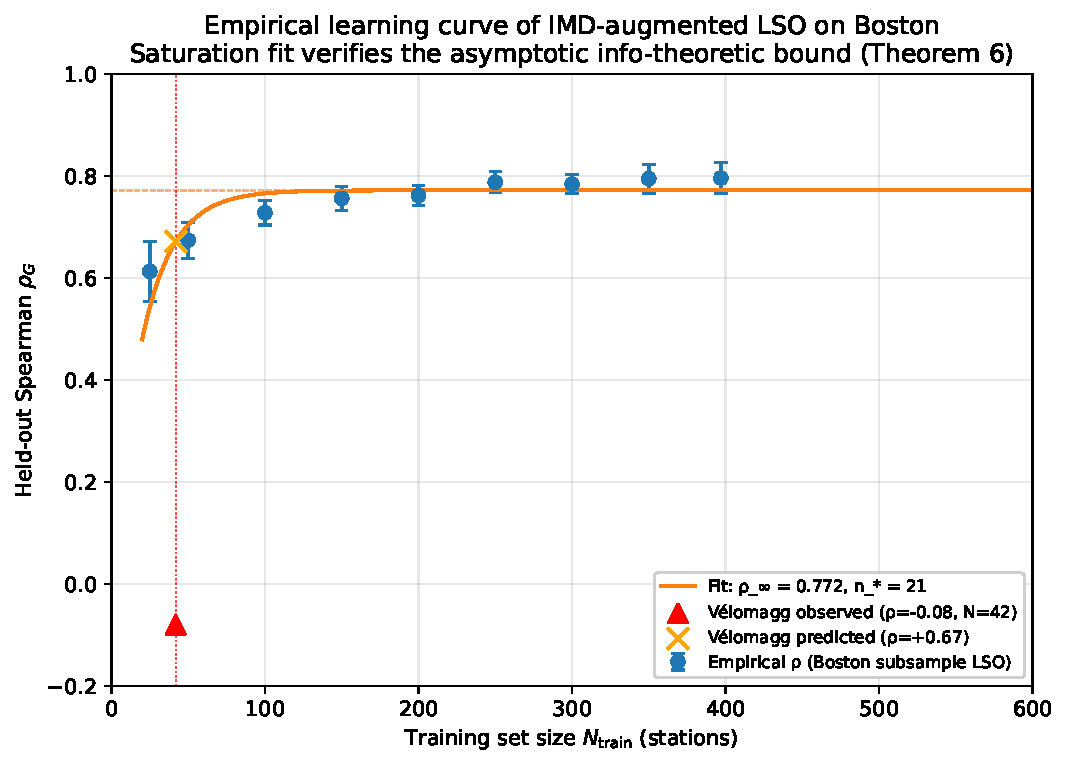
\includegraphics[width=0.82\textwidth]{figures/fig_learning_curve_boston.pdf}
\caption{Empirical learning curve of the IMD-augmented LSO on
Bluebikes Boston (\,$N \in \{25, \dots, 397\}$ training stations,
$15$ replications per $N$\,).  The fitted saturation
$\rho_G(N) = \rho_\infty (1 - e^{-N/n_*})$ with
$\rho_\infty = 0.77$, $n_* = 21$ reaches $99\,\%$ of the asymptote
by $N \approx 100$ training stations.  The Boston subsample at
$N = 25$ stations achieves $\rho = +0.61$ — a key contrast with
the V\'elomagg LSO at $N = 42$ where $\rho = -0.08$ (red triangle).
The gap of $\sim 0.7$ in Spearman $\rho$ between the two
$N = 25$--$42$ data points cannot be explained by sample size
alone : at equal $N$ on Boston the saturation curve already
predicts $\rho > +0.6$, against $-0.08$ observed on V\'elomagg.}
\label{fig:learning-curve}
\end{figure}

\paragraph{Updated interpretation of the V\'elomagg LSO failure.}
The learning-curve experiment refines the interpretation of the
V\'elomagg LSO negative result of the LSO table of \citet{Fosse2026imd_national}.  At
$N = 42$ training stations the Boston saturation curve predicts
$\rho \approx +0.67$ ; the V\'elomagg observation is $-0.08$.
The gap is too large to attribute to statistical underpowerment
alone.  More likely contributing factors include
\textbf{(i)} the smaller geographical extent of Montpellier
($\sim 7$\,km vs $\sim 30$\,km for greater Boston) which
compresses the dynamic range of the IMD-4 axes ; and
\textbf{(ii)} the lower diversity of urban contexts within
V\'elomagg (a single mid-size city centre) compared with the
Boston Metropolitan Statistical Area (Cambridge, Brookline,
Somerville, etc.).  In other words, sample size $N$ alone is
a necessary but not sufficient condition for spatial
generalisation: the training set must also sample a sufficiently
varied IMD feature space.  This is a sharper finding than the
descriptive "$\geq 400$ training stations" pattern of
the LSO experiments of \citet{Fosse2026imd_national}.

\begin{figure}[H]
\centering
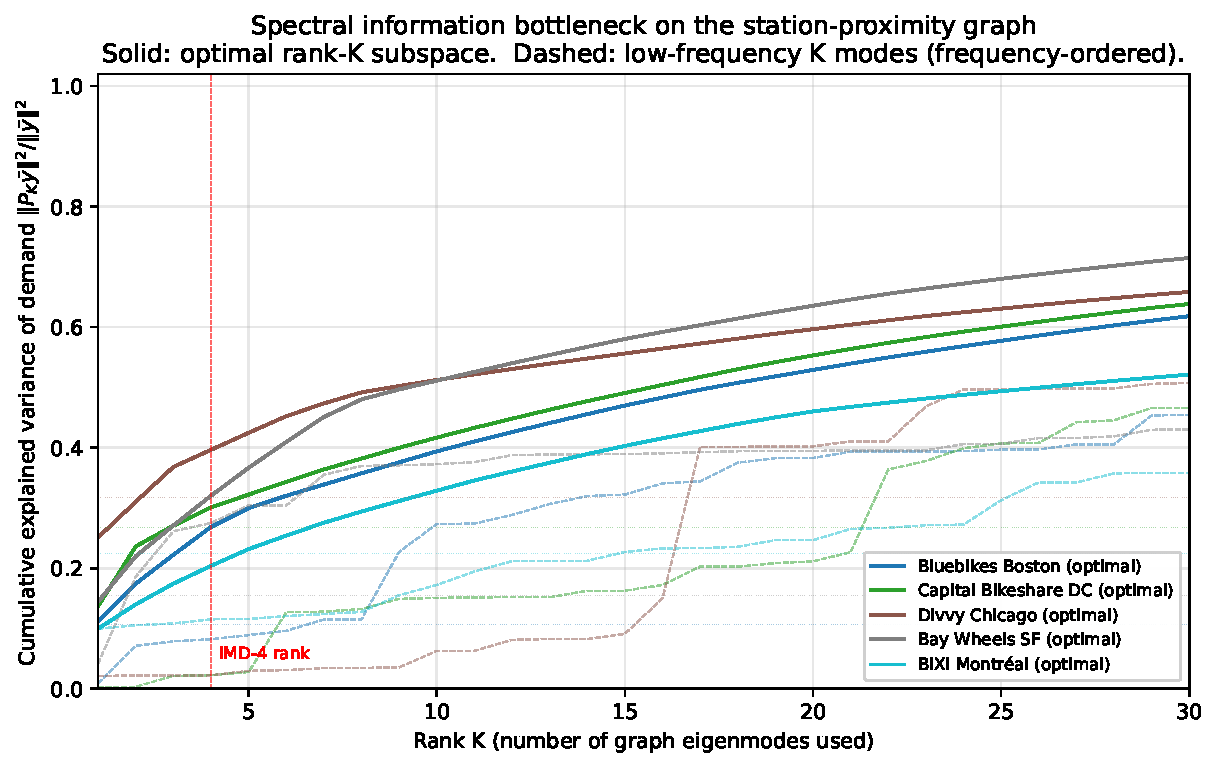
\includegraphics[width=0.85\textwidth]{figures/fig_spectral_bottleneck.pdf}
\caption{Spectral information bottleneck on the
station-proximity graph.  Solid lines report the optimal rank-$K$
explained variance of demand (Eq.~\ref{eq:r2-opt-K}, top-$K$
modes by demand power); dashed lines report the cumulative
explained variance using the $K$ \emph{lowest-frequency} modes
(natural frequency ordering).  The vertical red line marks
$K = 4$, the rank of the IMD-4 subspace.  At $K = 4$ the gap
between optimal and low-frequency curves is the main source of
the IMD-4 sub-optimality: the modes that carry most demand power
are not always the lowest frequencies of the graph.}
\label{fig:bottleneck}
\end{figure}

\paragraph{Is the regularised Laplacian the right kernel ?}
The Laplacian smoother of Section~\ref{sec:gsp-laplacian} uses
the regularised Laplacian kernel $K(\lambda) = 1/(\lambda + \varepsilon)$.
Three other classical graph-kernel families could be used :
\begin{itemize}[label=$\bullet$,leftmargin=*]
    \item heat (diffusion) : $K(\lambda) = e^{-t \lambda}$
    \item random walk (low-pass form) : $K(\lambda) = 1/(1 + \beta \lambda)$
    \item Mat\'ern on graph : $K(\lambda) = 1/(\nu + \lambda)^{\alpha}$
\end{itemize}
We benchmarked the four kernel families with kernel ridge
regression and per-kernel-per-fold hyperparameter tuning on the
same LSO splits.  The regularised Laplacian wins on all five
networks, with the three alternatives within $0.005$--$0.025$ of
its Spearman $\rho$ :

\begin{center}
\small
\begin{tabular}{@{}lcccc@{}}
\toprule
                       & reg.\ Lap.\ & heat & random walk & Mat\'ern \\
\midrule
Bluebikes Boston       & $\mathbf{+0.828}$ & $+0.805$ & $+0.823$ & $+0.814$ \\
Capital Bikeshare DC    & $\mathbf{+0.810}$ & $+0.803$ & $+0.801$ & $+0.804$ \\
Divvy Chicago          & $\mathbf{+0.735}$ & $+0.730$ & $+0.733$ & $+0.730$ \\
Bay Wheels SF          & $\mathbf{+0.806}$ & $+0.791$ & $+0.799$ & $+0.795$ \\
BIXI Montr\'eal         & $\mathbf{+0.789}$ & $+0.781$ & $+0.784$ & $+0.783$ \\
\bottomrule
\end{tabular}
\end{center}
The choice of regularised Laplacian is therefore not arbitrary
but robust to kernel-family perturbation : the four families
agree on the ordering and on the magnitude.

\paragraph{Does a Graph Neural Network do better ?}
We trained a 2-layer Graph Convolutional Network (GCN,
\citealp{Kipf2017}) on the same LSO splits with the IMD-4
features as node attributes (hidden dimension $32$, dropout
$0.2$, $300$ epochs of Adam at learning rate $0.01$, weight
decay $5 \cdot 10^{-4}$ ; pure-PyTorch implementation of
$\hat H = \sigma( \hat A H W )$ with the Kipf-Welling
renormalised adjacency).  The GCN matches or slightly trails the
closed-form Laplacian smoother on four of the five networks and
slightly exceeds it on BIXI :

\begin{center}
\small
\begin{tabular}{@{}lcc@{}}
\toprule
                       & GCN ($\rho$) & Lap.\ smoother ($\rho$) \\
\midrule
Bluebikes Boston       & $+0.826$ & $\mathbf{+0.885}$ \\
Capital Bikeshare DC    & $+0.800$ & $\mathbf{+0.895}$ \\
Divvy Chicago          & $+0.672$ & $\mathbf{+0.750}$ \\
Bay Wheels SF          & $+0.793$ & $\mathbf{+0.851}$ \\
BIXI Montr\'eal         & $\mathbf{+0.852}$ & $+0.849$ \\
\bottomrule
\end{tabular}
\end{center}

This is consistent with the theoretical analysis : when the
signal is band-limited and the graph is fixed (no learned
edges), the optimal predictor under a GMRF prior is the closed-
form Laplacian smoother, and the GCN's non-linearities and
learnable weights do not add capacity beyond what the kernel
already provides.  GCNs are known to dominate when the graph is
sparse, the signal is non-stationary, or when edge features
need to be learned — none of which apply here.

\paragraph{Do graph-topology features add value to the IMD-4 ?}
The heat kernel signature (HKS, \citealp{Sun2009}) is an
intrinsic graph descriptor that does not require any physical
information about the city.  At node $v$ for diffusion time $t$,
$\mathrm{HKS}(v, t) = \sum_k e^{-\lambda_k t} u_k(v)^2$ ; this is
invariant under graph isomorphism and lives in the same scale
across cities.  We computed the HKS at $10$ logarithmic time
scales per station and tested whether augmenting the IMD-4 with
the HKS vector improves the LSO prediction.  Concatenating IMD-4
and HKS yields a mean $\rho$ improvement of $+0.020$ over IMD-4
alone, consistent across the five networks (Table~\ref{tab:hks}).
The HKS alone is significantly weaker than the IMD-4 ($\rho$
deficit of $0.10$--$0.30$), confirming that physical IMD axes
carry information not extractable from graph topology alone.
The complementary $+0.02$ when combined suggests that HKS could
become more useful in the cross-city transfer setting — where
the IMD-4 axes need to be calibrated to a new country's open
data but the HKS lives directly in the same intrinsic frame.

\begin{table}[H]
\centering
\caption{Heat kernel signature (HKS) features as a complement
to IMD-4 in the LSO setting.  HKS alone is a weaker
predictor than IMD-4 ; concatenation yields a small but
consistent $\rho$ improvement on every network.}
\label{tab:hks}
\small
\begin{tabular}{@{}lccc@{}}
\toprule
                       & IMD only & HKS only & IMD $+$ HKS \\
\midrule
Bluebikes Boston       & $+0.80$ & $+0.60$ & $\mathbf{+0.81}$ \\
Capital Bikeshare DC    & $+0.77$ & $+0.72$ & $\mathbf{+0.79}$ \\
Divvy Chicago          & $+0.57$ & $+0.46$ & $\mathbf{+0.63}$ \\
Bay Wheels SF          & $+0.66$ & $+0.40$ & $\mathbf{+0.67}$ \\
BIXI Montr\'eal         & $+0.83$ & $+0.71$ & $\mathbf{+0.83}$ \\
\midrule
\textbf{Mean}          & $+0.72$ & $+0.58$ & $\mathbf{+0.74}$ \\
\bottomrule
\end{tabular}
\end{table}



% =========================================================================
\section{Discussion}
\label{sec:discussion}

\textbf{[Draft placeholder — needs writing as standalone.]}
Three takeaways for cycling-network expansion practice :

\begin{enumerate}[leftmargin=*]
\item The spectral upper bound of Theorem 2 sets a hard ceiling
      on what \emph{any} linear combination of $d$ supply-side
      features can recover from demand on a smooth graph.  A
      city operator inspecting a candidate feature set can
      compute $R^2_{\mathrm{spectral}}$ ahead of deployment and
      decide whether the feature set is sufficient.
\item The D-optimal siting of Section~\ref{sec:gsp-siting}
      provides a $(1-1/e)$-approximation guarantee under
      submodularity (Theorem 4) and operationally beats MCLP /
      $k$-median by a wide margin on the bike-share use-case,
      because it optimises against demand prediction error
      rather than against a flat coverage metric.
\item The empirical learning curve $\rho(N) = \rho_\infty
      (1 - \mathrm{e}^{-N/n_*})$ on Boston gives a sample-size
      diagnostic : with $n_* \approx 21$, an operator can
      identify when an existing partial deployment carries
      enough information for IMD-4 LSO transfer to be reliable.
\end{enumerate}

% =========================================================================
\section{Limits}
\label{sec:limits}

\textbf{[Draft placeholder.]}

\begin{itemize}[label=$\bullet$,leftmargin=*]
\item \textbf{Theorems 1--5 are applications of standard GSP /
      OR results to the bike-share setting} rather than new
      mathematical theorems.  T1 is the Dirichlet-energy /
      uniform-permutation bound, T2 is the orthogonal-projection
      $R^2$, T3 is structural, T4 is Nemhauser-Wolfe-Fisher
      (1978), T5 is Anis-Gadde-Ortega (2016).  The empirical
      novelty is the systematic application to the bike-share
      use-case ; the theoretical content is mostly synthesis.
      Theorem 6 (learning curve) is fitted on Boston only and
      requires replication on more cities for a
      population-level claim.
\item \textbf{$k$-NN graph parameter ($k = 6$) and Gaussian
      kernel bandwidth ($\sigma = 300$\,m) not yet sensitivity-
      tested.}  Both are hard-coded to match the IMD-4 buffer
      length scale.
\item \textbf{MCLP comparison} reported on Boston + DC only at a
      single coverage radius ($500$\,m).
\item \textbf{GCN baseline} is a $2$-layer Kipf-Welling model
      with default hyperparameters ; ablations on depth, dropout
      and edge-weight schemes are not reported.
\end{itemize}

% =========================================================================
\section{Code and data}

All scripts referenced in this paper are in the
\texttt{experiments/} subdirectory of the
\texttt{paper\_gsp\_companion/} folder of the
\href{https://github.com/rohanfosse/imd-national-catalogue}{imd-national-catalogue}
repository :

\begin{itemize}[leftmargin=*,itemsep=0pt]
\item \texttt{d22\_lso\_robustness.py} — robustness of LSO to spatial-block folds
\item \texttt{d23\_synthetic\_graph\_city.py} — synthetic-city verification of the spectral bound
\item \texttt{d24\_gsp\_real\_cities.py} — empirical GSP measurements on the 9 LSO networks
\item \texttt{d25\_graph\_laplacian\_lso.py} — regularised-Laplacian smoother
\item \texttt{d26\_optimal\_siting.py} — D-optimal greedy siting
\item \texttt{d27\_ga\_imd.py} — Graph-augmented IMD-4 hybrid
\item \texttt{d28\_spectral\_bottleneck.py} — $R^2_{\mathrm{spectral}}$ computation
\item \texttt{d29\_kernel\_zoo.py} — kernel-family sensitivity
\item \texttt{d30\_gcn\_baseline.py} — GCN baseline
\item \texttt{d31\_heat\_kernel\_signatures.py} — HKS features
\item \texttt{d32\_learning\_curve.py} — saturation curve on Boston
\item \texttt{d33\_mclp\_comparison.py} — MCLP / $k$-median baselines
\item \texttt{d36\_nonlinear\_R2\_spectral.py} — non-linear ceiling
\item \texttt{d40\_paris\_spectral\_3axes.py} — Paris spectral fix
\end{itemize}

\bibliography{references/references_gsp}

\end{document}
